\documentclass[9pt, aspectratio=169]{beamer}
\mode<presentation>
\usepackage[T1]{fontenc}
\usepackage{color}
\usepackage{graphicx}
\usepackage{natbib}
\usepackage{tikz}
\usepackage{pgfplots}
\usetikzlibrary{spy,calc}
\usepackage{hyperref}
\usepackage{caption}
\usepackage{subcaption}
\usepackage{adjustbox}
\usepackage{appendixnumberbeamer}

\usepackage{tcolorbox}

\usetheme{Boadilla}


\definecolor{mcctext}{HTML}{0d77b0}
\definecolor{mcclogo}{HTML}{0067a1}
\definecolor{mcclight}{HTML}{D9E8F1}


\usecolortheme[named=mcclogo]{structure}


\usefonttheme{professionalfonts}

\title[Big Literature]{A Topography of Climate Change Research}
\subtitle{}
\author{Max Callaghan }
\institute[MCC]{
	{\footnotesize with Jan Minx, Piers Forster} \\ \medskip
	\includegraphics[height=1cm,width=2cm]{MCC_Logo_RZ_rgb.jpg} \hspace{3em}
	\includegraphics[height=1cm]{University-of-Leeds-logo.png}
}
\date{January 26, 2019}


\newtheorem*{remark}{}

\bibliographystyle{apalike}

\newif\ifblackandwhitecycle
\gdef\patternnumber{0}

\pgfkeys{/tikz/.cd,
	zoombox paths/.style={
		draw=orange,
		very thick
	},
	black and white/.is choice,
	black and white/.default=static,
	black and white/static/.style={ 
		draw=white,   
		zoombox paths/.append style={
			draw=white,
			postaction={
				draw=black,
				loosely dashed
			}
		}
	},
	black and white/static/.code={
		\gdef\patternnumber{1}
	},
	black and white/cycle/.code={
		\blackandwhitecycletrue
		\gdef\patternnumber{1}
	},
	black and white pattern/.is choice,
	black and white pattern/0/.style={},
	black and white pattern/1/.style={    
		draw=white,
		postaction={
			draw=black,
			dash pattern=on 2pt off 2pt
		}
	},
	black and white pattern/2/.style={    
		draw=white,
		postaction={
			draw=black,
			dash pattern=on 4pt off 4pt
		}
	},
	black and white pattern/3/.style={    
		draw=white,
		postaction={
			draw=black,
			dash pattern=on 4pt off 4pt on 1pt off 4pt
		}
	},
	black and white pattern/4/.style={    
		draw=white,
		postaction={
			draw=black,
			dash pattern=on 4pt off 2pt on 2 pt off 2pt on 2 pt off 2pt
		}
	},
	zoomboxarray inner gap/.initial=5pt,
	zoomboxarray columns/.initial=2,
	zoomboxarray rows/.initial=2,
	subfigurename/.initial={},
	figurename/.initial={zoombox},
	zoomboxarray/.style={
		execute at begin picture={
			\begin{scope}[
				spy using outlines={%
					zoombox paths,
					width=\imagewidth / \pgfkeysvalueof{/tikz/zoomboxarray columns} - (\pgfkeysvalueof{/tikz/zoomboxarray columns} - 1) / \pgfkeysvalueof{/tikz/zoomboxarray columns} * \pgfkeysvalueof{/tikz/zoomboxarray inner gap} -\pgflinewidth,
					height=\imageheight / \pgfkeysvalueof{/tikz/zoomboxarray rows} - (\pgfkeysvalueof{/tikz/zoomboxarray rows} - 1) / \pgfkeysvalueof{/tikz/zoomboxarray rows} * \pgfkeysvalueof{/tikz/zoomboxarray inner gap}-\pgflinewidth,
					magnification=3,
					every spy on node/.style={
						zoombox paths
					},
					every spy in node/.style={
						zoombox paths
					}
				}
				]
			},
			execute at end picture={
			\end{scope}
			\node at (image.north) [anchor=north,inner sep=0pt] {\subcaptionbox{\label{\pgfkeysvalueof{/tikz/figurename}-image}}{\phantomimage}};
			\node at (zoomboxes container.north) [anchor=north,inner sep=0pt] {\subcaptionbox{\label{\pgfkeysvalueof{/tikz/figurename}-zoom}}{\phantomimage}};
			\gdef\patternnumber{0}
		},
		spymargin/.initial=0.5em,
		zoomboxes xshift/.initial=1,
		zoomboxes right/.code=\pgfkeys{/tikz/zoomboxes xshift=1},
		zoomboxes left/.code=\pgfkeys{/tikz/zoomboxes xshift=-1},
		zoomboxes yshift/.initial=0,
		zoomboxes above/.code={
			\pgfkeys{/tikz/zoomboxes yshift=1},
			\pgfkeys{/tikz/zoomboxes xshift=0}
		},
		zoomboxes below/.code={
			\pgfkeys{/tikz/zoomboxes yshift=-1},
			\pgfkeys{/tikz/zoomboxes xshift=0}
		},
		caption margin/.initial=4ex,
	},
	adjust caption spacing/.code={},
	image container/.style={
		inner sep=0pt,
		at=(image.north),
		anchor=north,
		adjust caption spacing
	},
	zoomboxes container/.style={
		inner sep=0pt,
		at=(image.north),
		anchor=north,
		name=zoomboxes container,
		xshift=\pgfkeysvalueof{/tikz/zoomboxes xshift}*(\imagewidth+\pgfkeysvalueof{/tikz/spymargin}),
		yshift=\pgfkeysvalueof{/tikz/zoomboxes yshift}*(\imageheight+\pgfkeysvalueof{/tikz/spymargin}+\pgfkeysvalueof{/tikz/caption margin}),
		adjust caption spacing
	},
	calculate dimensions/.code={
		\pgfpointdiff{\pgfpointanchor{image}{south west} }{\pgfpointanchor{image}{north east} }
		\pgfgetlastxy{\imagewidth}{\imageheight}
		\global\let\imagewidth=\imagewidth
		\global\let\imageheight=\imageheight
		\gdef\columncount{1}
		\gdef\rowcount{1}
		\gdef\zoomboxcount{1}
	},
	image node/.style={
		inner sep=0pt,
		name=image,
		anchor=south west,
		append after command={
			[calculate dimensions]
			node [image container,subfigurename=\pgfkeysvalueof{/tikz/figurename}-image] {\phantomimage}
			node [zoomboxes container,subfigurename=\pgfkeysvalueof{/tikz/figurename}-zoom] {\phantomimage}
		}
	},
	color code/.style={
		zoombox paths/.append style={draw=#1}
	},
	connect zoomboxes/.style={
		spy connection path={\draw[draw=none,zoombox paths] (tikzspyonnode) -- (tikzspyinnode);}
	},
	help grid code/.code={
		\begin{scope}[
			x={(image.south east)},
			y={(image.north west)},
			font=\footnotesize,
			help lines,
			overlay
			]
			\foreach \x in {0,1,...,9} { 
				\draw(\x/10,0) -- (\x/10,1);
				\node [anchor=north] at (\x/10,0) {0.\x};
			}
			\foreach \y in {0,1,...,9} {
				\draw(0,\y/10) -- (1,\y/10);                        \node [anchor=east] at (0,\y/10) {0.\y};
			}
		\end{scope}    
	},
	help grid/.style={
		append after command={
			[help grid code]
		}
	},
}

\newcommand\phantomimage{%
	\phantom{%
		\rule{\imagewidth}{\imageheight}%
	}%
}
\newcommand\zoombox[2][]{
	\begin{scope}[zoombox paths]
		\pgfmathsetmacro\xpos{
			(\columncount-1)*(\imagewidth / \pgfkeysvalueof{/tikz/zoomboxarray columns} + \pgfkeysvalueof{/tikz/zoomboxarray inner gap} / \pgfkeysvalueof{/tikz/zoomboxarray columns} ) + \pgflinewidth
		}
		\pgfmathsetmacro\ypos{
			(\rowcount-1)*( \imageheight / \pgfkeysvalueof{/tikz/zoomboxarray rows} + \pgfkeysvalueof{/tikz/zoomboxarray inner gap} / \pgfkeysvalueof{/tikz/zoomboxarray rows} ) + 0.5*\pgflinewidth
		}
		\edef\dospy{\noexpand\spy [
			#1,
			zoombox paths/.append style={
				black and white pattern=\patternnumber
			},
			every spy on node/.append style={#1},
			x=\imagewidth,
			y=\imageheight
			] on (#2) in node [anchor=north west] at ($(zoomboxes container.north west)+(\xpos pt,-\ypos pt)$);}
		\dospy
		\pgfmathtruncatemacro\pgfmathresult{ifthenelse(\columncount==\pgfkeysvalueof{/tikz/zoomboxarray columns},\rowcount+1,\rowcount)}
		\global\let\rowcount=\pgfmathresult
		\pgfmathtruncatemacro\pgfmathresult{ifthenelse(\columncount==\pgfkeysvalueof{/tikz/zoomboxarray columns},1,\columncount+1)}
		\global\let\columncount=\pgfmathresult
		\ifblackandwhitecycle
		\pgfmathtruncatemacro{\newpatternnumber}{\patternnumber+1}
		\global\edef\patternnumber{\newpatternnumber}
		\fi
	\end{scope}
}


\begin{document}
	
\begin{frame}
	\titlepage
\end{frame}

\addtobeamertemplate{frametitle}{}{
	\begin{tikzpicture}[remember picture,overlay]
	\node[anchor=north east,yshift=2pt] at (current page.north east) {\includegraphics[height=0.6cm]{MCC_Logo_RZ_rgb.jpg}};
	\end{tikzpicture}}

\begin{frame}{Introduction}
\begin{columns}[T]
	\begin{column}{0.4\linewidth}
		\begin{center}
			\begin{figure}
				\includegraphics[width=1\linewidth]{../plots/Hondius_Portrait_of_map-makers}
				\caption{Portrait of map-makers, Gerardus Mercator and Jodocus Hondius (Jodocus Hondius) source: Wikipedia Commons}
			\end{figure}
		\end{center}
	\end{column}
	\begin{column}{0.6\linewidth}
		%\begin{minipage}{0.9\linewidth}
			\begin{columns}[t]
				\begin{column}{0.45\linewidth}<2->
					\begin{figure}
						\includegraphics[width=0.6\linewidth]{syrcover}
					\end{figure}
				\end{column}
				\begin{column}{0.45\linewidth}<2->
					\begin{itemize}
						\item<2-> The IPCC has a \textit{cartographic} role at the science policy interface \citep{Edenhofer2014, Edenhofer2015}
						\item<3-> It is much studied in STS \citep{Hulme2010}
					\end{itemize}
				\end{column}
			\end{columns}
		%\end{minipage}
		\bigskip
		\begin{center}
			\begin{itemize}
				\item<4-> A topography is a description of a landscape
				\item<5-> Topics (from the Greek ``topos'', place) can describe the features of a body of text
			\end{itemize}
		\end{center}
	\end{column}
\end{columns}
\end{frame}

\begin{frame}{Outline}
\tableofcontents
\end{frame}

\section{Motivation}
\frame{\tableofcontents[currentsection]}

\begin{frame}{Context - Big Literature}
\begin{columns}
	\begin{column}{0.618\linewidth} % Golden ratio columns
		\begin{figure}
			\includegraphics[width=\linewidth]{../plots/literature_size/pubs_time_wgb_lp.pdf}
			\caption{Articles on climate change in the Web of Science}
		\end{figure}
	\end{column}
	\begin{column}{0.382\linewidth}
		A challenge for
		\begin{itemize}
			\item Global environmental assessments
			\item Our understanding of global environmental assessments
			\item Evidence synthesis more generally
		\end{itemize}
	\end{column}
\end{columns}
\end{frame}

\begin{frame}{The IPCC in the age of Big Literature}

\begin{columns}
	\begin{column}{0.382\linewidth}
		\begin{itemize}
			\item<1->We entrust the IPCC with providing a \textit{comprehensive} and \textit{transparent} assessment of the literature 
			\item<2->Although IPCC reports cite ever greater numbers of papers, this number decreases in proportion to the number of papers in literature
			
		\end{itemize}
	\end{column}
	\begin{column}{0.618\linewidth}<2->
		\begin{figure}
			\includegraphics[width=\linewidth]{wos_IPCC_shares.png}
			\caption{\citep{Minx2017l}}
		\end{figure}
	\end{column}
\end{columns}

\end{frame}

%%%%%%%%%%%%%%%%%%%%%%%%%%%%%%%%%%%%%%%

\begin{frame}{What Do We Know About the IPCC?}
\begin{columns}
	\begin{column}{0.618\linewidth}
		\begin{itemize}
			\item<2-> The social sciences are seen as under-represented in IPCC reports
			\item<3-> \citep{Bjurstroem2011} are often cited as evidence of this under-representation, e.g. as demonstrating ``a powerful bias to the natural sicences in the construction of `IPCC knowledge' '' \cite{Hulme2010}
			\item<4-> The evidence is simply the relative shares of the different disciplines in IPCC citations
			
		\end{itemize}
	\end{column}
	\begin{column}{0.382\linewidth}<2->
		\begin{figure}[h!]
			\begin{center}
				\includegraphics[width=0.85\linewidth]{../plots/victor.png}
				\caption{\citep{Victor2015}}
			\end{center}
		\end{figure}
	\end{column}
\end{columns}
\end{frame}

\begin{frame}{The Age of Climate Solutions? }
\begin{columns}
	
	\begin{column}{0.618\linewidth}<1->
		\begin{figure}[h!]
			\begin{center}
				\includegraphics[width=\linewidth]{../plots/kowarsch-solutions.png}
				\caption{\citep{Kowarsch2017}}
			\end{center}
		\end{figure}
		
	\end{column}
	\begin{column}{0.382\linewidth}
		\begin{itemize}
			\item<1-> Demand for solutions is increasing
			\item<2-> We know little about the supply of solutions in the literature
			
			
		\end{itemize}
	\end{column}
\end{columns}
\end{frame}


\section{Methods}
\frame{\tableofcontents[currentsection]}

\begin{frame}{Investigating bibliometric and text data}

To understand the representation of social science and solutions relevant knowledge in IPCC reports, we look at journal classification and document abstracts

\bigskip

\textbf{Data:}

400,000 papers on climate change from the Web of Science (query following \cite{Grieneisen2011}), matched with 70,000 IPCC citations (Using Doc2Vec)

\bigskip

\textbf{Topic modelling:}

We use topic modelling (with NMF \citep{Lee1999}) to understand the thematic content of papers

\bigskip

\textbf{Topographic mapping:}

We project the documents' topical locations into 2 dimensions using t-SNE \citep{vandermaaten2008} 

\bigskip

\textbf{Measuring representation:}

We compare the proportions of categories of documents in the whole of the literature with the subset of the literature that is cited by the IPCC

\end{frame}


\begin{frame}{Words, words, words}

\begin{table}[h]
	\begin{adjustbox}{width=0.8\linewidth}
		\input{../tables/growth_table.tex}
	\end{adjustbox}			
	\caption{Growth in climate change literature}
	\label{growthtable}
\end{table}	

%		\begin{itemize}
%			\item bla
%			
%		\end{itemize}

Data from WoS Core Collection, query following \citet{Grieneisen2011}

\end{frame}


\begin{frame}{Approach - What is the matter?}

\begin{columns}
	\begin{column}{0.382\linewidth}
		\begin{itemize}
			\item<1-> Topic modelling \citep{Blei2012} describes a suite of algorithms to discover the latent semantic content of documents
			\item<2-> NMF \citep{Lee1999} is a dimensionality reduction technique that can be used for topic modelling
			\item<3-> Topics are distributions of words. They describe documents.
			\item<4-> A document's topic scores describe its association with each topic 
			
		\end{itemize}
	\end{column}
	\begin{column}{0.618\linewidth}<2->
		\only<2->{\(V_{i\mu} \) is a term frequency-inverse document frequency matrix of \textit{stemmed} terms} 
		\only<2->{\[V_{i\mu} \approx (WH)_{i\mu} = \sum_{a=1}^{r}W_{ia}H_{a\mu} \] \(V\) is approximated by the product of \(W\) and \(H\)}
		
		\begin{figure}
			\includegraphics[width=\linewidth]{../plots/VWH.png}
		\end{figure}
	\end{column}
	
\end{columns}

\end{frame}

\begin{frame}{Doc Topic Example}
\begin{figure}
	\includegraphics[width=0.8\linewidth]{../plots/single_doc_3_536594.pdf}
\end{figure}

\end{frame}

\section{Results}
\frame{\tableofcontents[currentsection]}

\begin{frame}[plain]{A Topography of Climate Change Literature}


\vspace{-0.5cm}

\begin{columns}
	\begin{column}{0.6\linewidth}<1->
		\begin{center}
			%\hspace{-1.3cm}
			\includegraphics[width=0.9\linewidth]{../tsne_results/plots/run_1861_s_0_p100_all_topic_words_oecds_lp.png}
		\end{center}
		
	\end{column}
	
	
	\begin{column}{0.4\linewidth}
		\begin{itemize}
			\item<1-> We use t-distributed stochastic neighbour embedding \citep{vandermaaten2008}
			to reduce documents' topic vectors to 2 dimensions  
			\item<2-> Each dot is a document, and documents with similar topic vectors are close together in the 2-dimensional space
			\item<3-> We can see the preponderance of natural sciences, and the greater or lesser clustering of disciplines in certain topic areas
			
			
		\end{itemize}
	\end{column}
\end{columns}

\end{frame}

\begin{frame}

\begin{figure}\centering
	\begin{tikzpicture}[zoomboxarray]
	\node [image node] { \includegraphics[width=0.45\textwidth]{../tsne_results/plots/run_1861_s_0_p100_all_topic_words_oecds_lp.png} };
	\zoombox[magnification=2.5]{0.35,0.7}
	\zoombox[magnification=2]{0.65,0.65}
	\zoombox[magnification=3]{0.15,0.4}
	\zoombox[magnification=3]{0.85,0.5}
	\end{tikzpicture}
\end{figure}

\end{frame}

\begin{frame}{The Social Sciences are No Longer Under-Represented in IPCC reports}
\begin{columns}
	
	\begin{column}{0.382\linewidth}
		\begin{itemize}
			\item<1-> The social sciences were under-represented in AR3, but by AR5 are over-represented
			\item<2-> The share of natural science documents in IPCC citations is similar to the share in the wider literature
			\item<3-> Agricultural sciences and engineering \& technology are under-represented		
		\end{itemize}
	\end{column}
	
	\begin{column}{0.618\linewidth}<1->
		\begin{figure}[h!]
			\begin{center}
				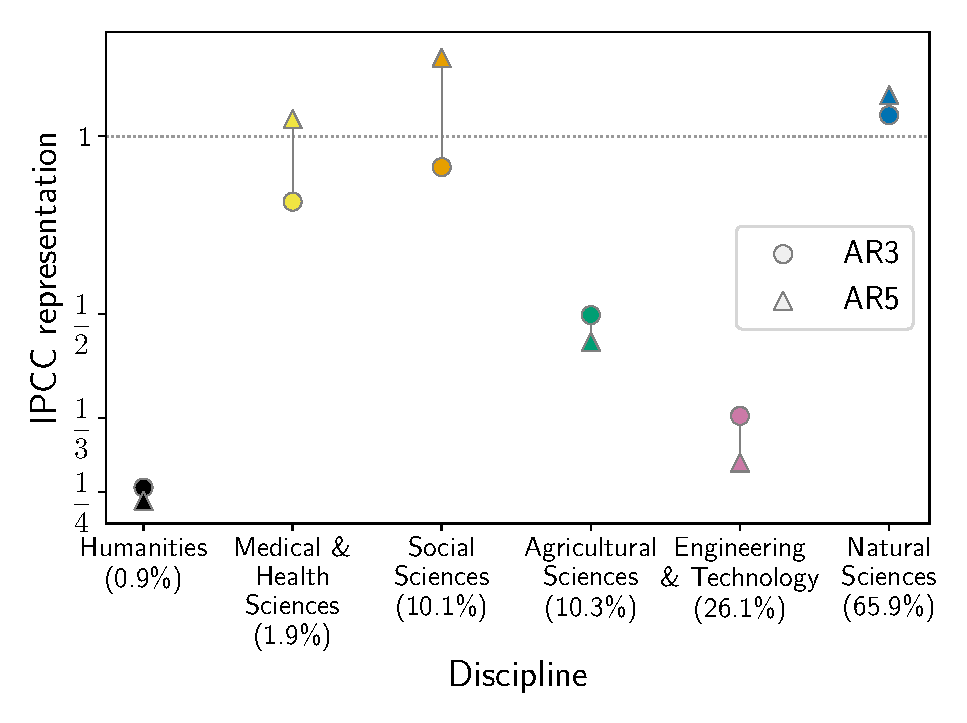
\includegraphics[width=\linewidth]{../plots_pub/ipcc_rep_oecds_simplified_lp.pdf}
			\end{center}
		\end{figure}
	\end{column}
\end{columns}
\end{frame}

\begin{frame}{Topics on solutions are newer and under-represented}

\vspace{-0.5cm}

\begin{columns}
	
	\begin{column}{0.618\linewidth}<1->
		\begin{figure}[h!]
			\begin{center}
				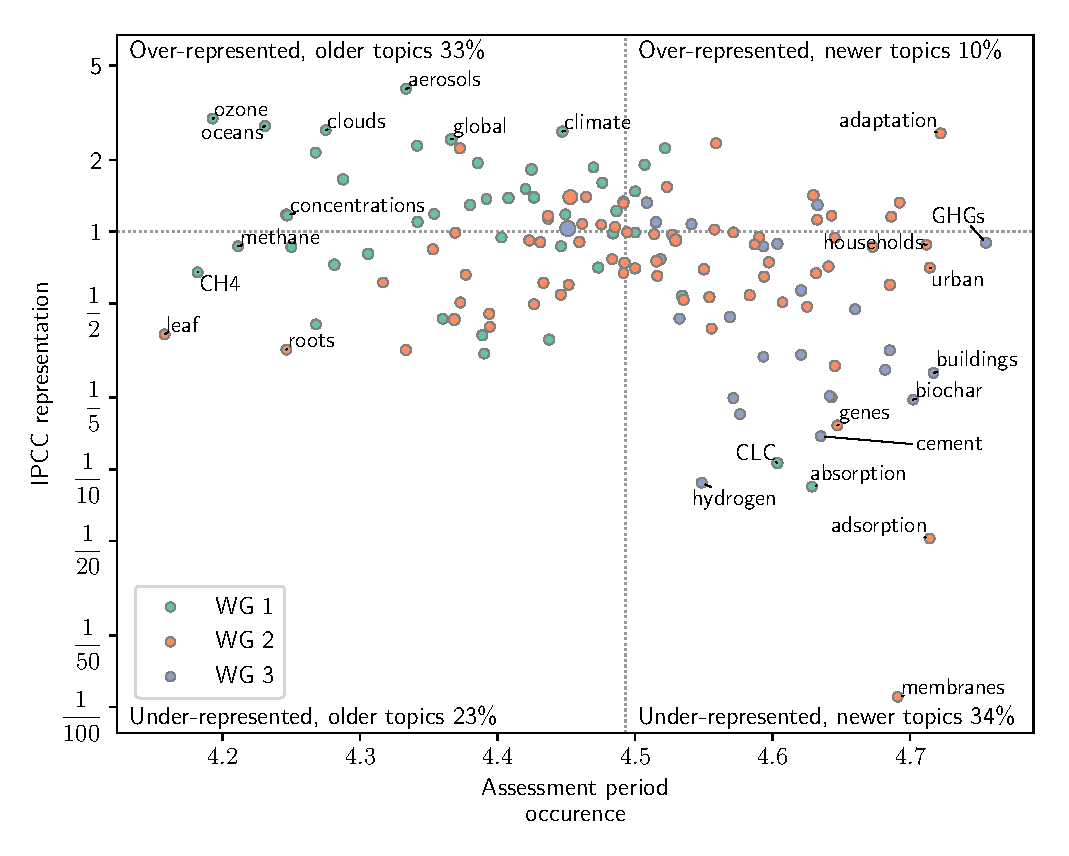
\includegraphics[width=\linewidth]{../plots_pub/rep_time_lp.pdf}
			\end{center}
		\end{figure}
		
	\end{column}
	\begin{column}{0.382\linewidth}
		\begin{itemize}
			\item<1-> The physical science of climate change is older and better covered
			\item<2-> Topics on ``solutions'' (although rather technical than policy) are newer and under-represented
			\item<3-> Newer WGII topics are better covered than newer WGIII topics
			
			
		\end{itemize}
	\end{column}
\end{columns}
\end{frame}

\begin{frame}{Topics on solutions are newer and under-represented}

\vspace{-0.5cm}

\begin{columns}
	
	\begin{column}{0.618\linewidth}<1->
		\begin{figure}[h!]
			\begin{center}
				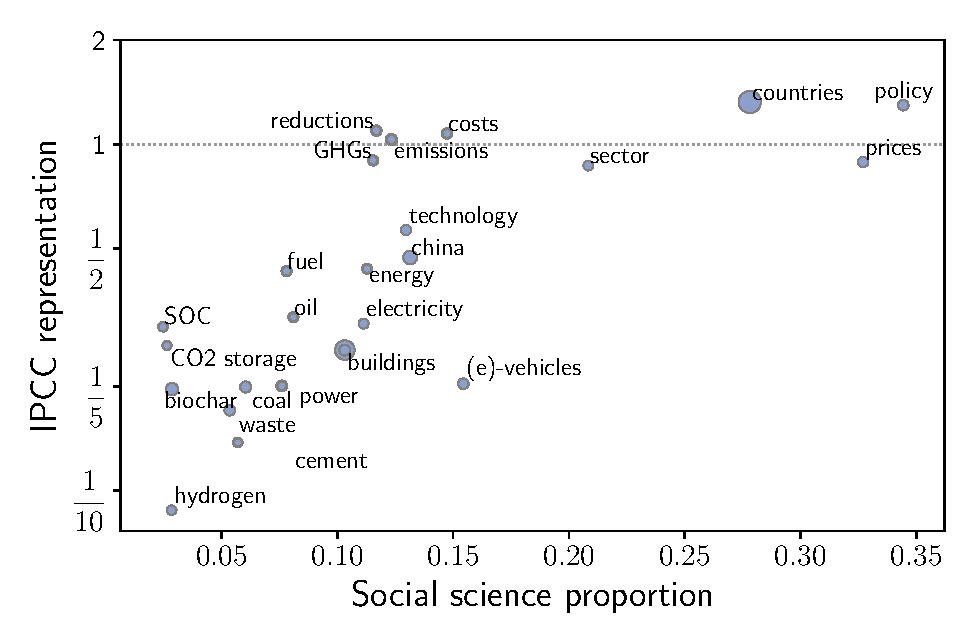
\includegraphics[width=\linewidth]{../plots/run_1861_wg3_socsci_lp.pdf}
			\end{center}
		\end{figure}
		
	\end{column}
	\begin{column}{0.382\linewidth}
		\begin{itemize}
			\item<1-> Technical solutions topics in WGIII contain little social science research and are under-represented
			
			
		\end{itemize}
	\end{column}
\end{columns}
\end{frame}

\begin{frame}{Conclusions}
\begin{columns}[t]
	\begin{column}{0.618\linewidth}
		\begin{itemize}
			\item<1-> Lack of social science knowledge in IPCC $ \neq $ IPCC natural science bias
			\item<2-> If there is a lack, we need to produce more social science knowledge, particularly on technical solutions
			\item<3-> There is a vast technical literature on solutions which is relatively untapped
		\end{itemize}
	
		\bigskip
		\bigskip
		\only<7->{
		\hrule
		\bigskip
		\bigskip
		\hspace{2em}A Topography of Climate Change Research
		\bigskip
		
		\hspace{2em}\url{https://dx.doi.org/10.1038/s41558-019-0684-5}
		
		\bigskip
		\hspace{2em}\url{callaghan@mcc-berlin.net}
		}
	\end{column}
	\begin{column}{0.382\linewidth}<4->
		\textbf{But,}
		\begin{itemize}
			\item<4-> Literature here is not all relevant climate knowledge (only WoS, only directly on climate change)
			\item<5-> Relative representation of different parts of the literature is job of IPCC to decide, not a computer
		\end{itemize}
		\only<6->{\textbf{Nevertheless,}}
		\begin{itemize}
			\item<6-> Computer assisted methods can help the IPCC make its decisions on how to represent the literature from a more solid basis, and efficiently point to areas of growth or of under-representation
		\end{itemize}
	\end{column}
\end{columns}
\end{frame}


\begin{frame}{Bibliography}
\scriptsize
\bibliography{../manuscript/Mendeley}
\end{frame}




%%%%%%%%%%%%%%%%%%%%%%%%%%%%%%%%%%
\appendix


\begin{frame}{n Topics}
\vspace{-0.4cm}September
\begin{figure}
	\includegraphics[width=1\linewidth]{../plots_pub/topic_rep_ks_wide.pdf}
\end{figure}

\end{frame}

%%%%%%%%%%%%%%%%%%%%%%%%%%%%%%%

\end{document}



\end{document}